\section{Użytkowanie}
%\subsection{Użytkownik}
Z punktu widzenia użytkownika (gracza) wszystko co należy zrobić to udać się pod adres www gdzie został udostępniony zasób znajdujący się w katalogu \emph{frontend} kodu źródłowego. Intuicyjny interfejs sam poprowadzi gracza

Na rysunku \ref{fig:login} zamieszczono zrzut ukazujący panel logowania istniejącego użytkownika. Na ekranie tym widnieje również odnośnik pozwalający na rejestrację nowego użytkownika.

\begin{figure}[h]
    \centering
    
\includegraphics[width=0.9\textwidth]{imgs/login.png}
    \caption{Widok ekranu logowania.}
    \label{fig:login}
\end{figure}

Ekran przedstawiony na rysunku \ref{fig:register} pokazuje wygląd ekranu do rejestracji nowego użytkownika.

\begin{figure}[h]
    \centering
    
\includegraphics[width=0.9\textwidth]{imgs/register.png}
    \caption{Rejestracja.}
    \label{fig:register}
\end{figure}
Rysunek \ref{fig:error-example} pokazuje widok wiadomości przykładowego błędu. W tym przypadku system informuje nas o tym, że nazwa użytkownika jest już zajęta.

\begin{figure}[h]
    \centering
    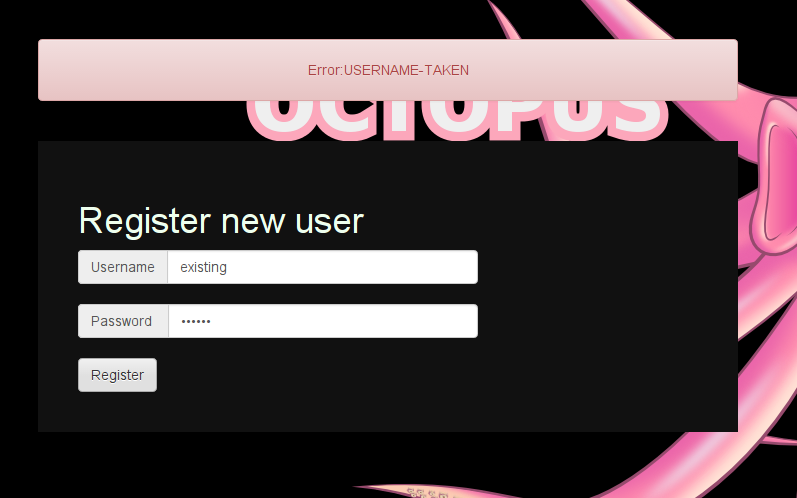
\includegraphics[width=0.9\textwidth]{imgs/error.png}
    \caption{Przykładowy błąd.}
    \label{fig:error-example}
\end{figure}
\clearpage
Po udanym zalogowaniu użytkownikowi pokaże się widok dostępny dla zalogowanych. W górnej części widać listę dostępnych kanałów, niżej panel do tworzenia nowych oraz przyciski \emph{Logout} i \ref{fig:zone} służące odpowiednio do wylogowania i odświeżenia listy kanałów, lista kanałów odświeża się również samoczynnie.

\begin{figure}[h]
    \centering
    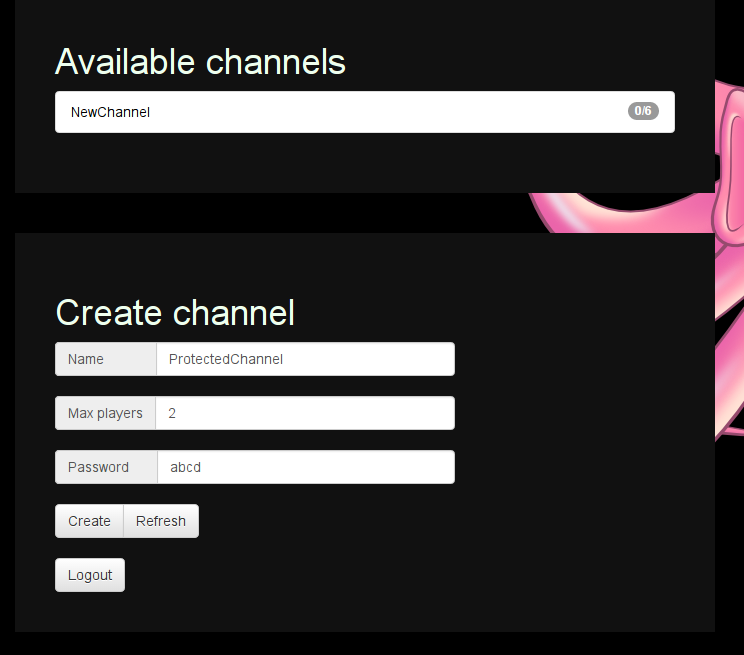
\includegraphics[width=0.9\textwidth]{imgs/beforeCreation.png}
    \caption{Strefa zalogowanego użytkownika.}
    \label{fig:zone}
\end{figure}
\clearpage
Na rysunku \ref{fig:chans} widać, jak reprezentowane są kanały z hasłem, obok ilości dostępnego miejsca na kanale, widnieje symbol kłódki.


\begin{figure}[h]
    \centering
    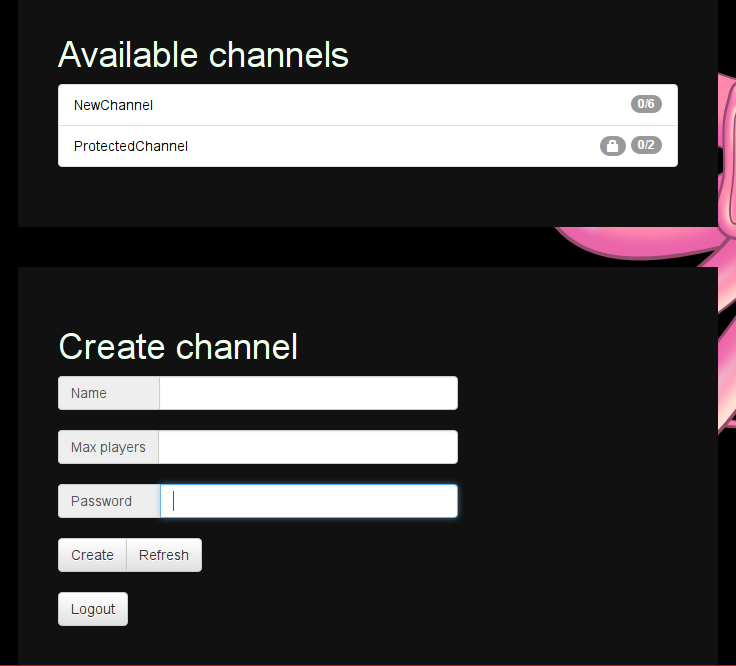
\includegraphics[width=0.9\textwidth]{imgs/twoChannels.png}
    \caption{Widok przedstawia listę dwóch kanałów na serwerze.}
    \label{fig:chans}
\end{figure}
\clearpage
Rysunek \ref{fig:game} prezentuje widok rozgrywki.
\begin{figure}[h]
    \centering
    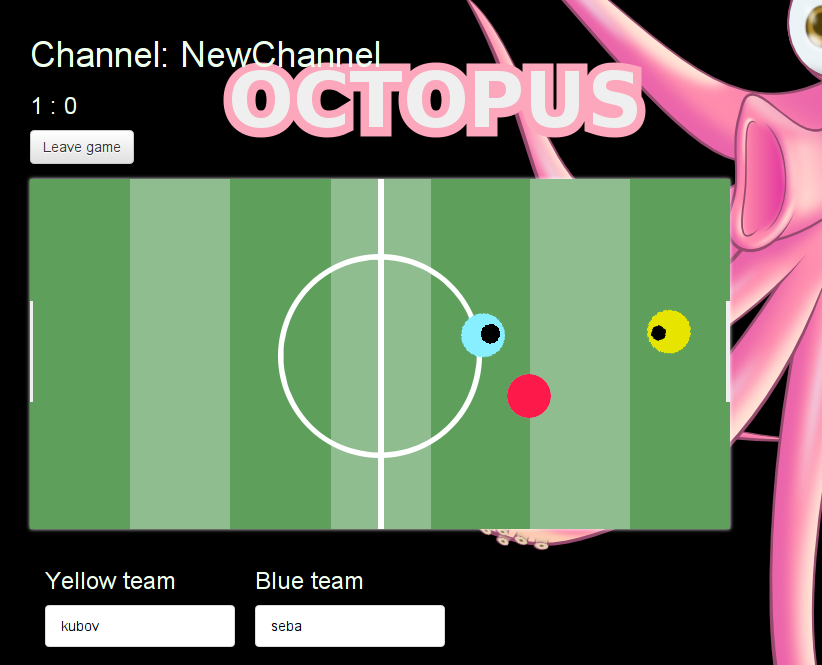
\includegraphics[width=0.9\textwidth]{imgs/gameView.png}
    \caption{Widok rozgrywki}
    \label{fig:game}
\end{figure}






%% \subsection{Dla administartora}
%% Posiadając system Linux bez trudu można uruchomić własny serwer gry korzystając z polecenia: \begin{verbatim}
%%   sbcl --load "backend/run-octopus.lisp"
%%   \end{verbatim}
%% Wymaganiem oczywiście jest posiadanie 
